\section{Watermark performance
evaluation}\label{watermark-performance-evaluation}

\textbf{Martino Ferrari}

\subsection{Non-blind watermark
detection}\label{non-blind-watermark-detection}

\paragraph{Exercise 1.1}\label{exercise-1.1}

For the given hypotesis:

\[
\begin{cases}
    \mathcal{H}_0:\quad v = x+z \\
    \mathcal{H}_1:\quad v = x+w+z
\end{cases}
\]

where \(x\) is the host image, \(w\) is the watermark and \(z\) is a
noise with distribution: \(\mathcal{N}(0,\sigma_{noise}^2)\).\\
Compute numerically the following property:

\begin{itemize}
\tightlist
\item
  \(P_f\)
\item
  \(P_m\)
\item
  \(P_d\)
\end{itemize}

\begin{figure}
\centering
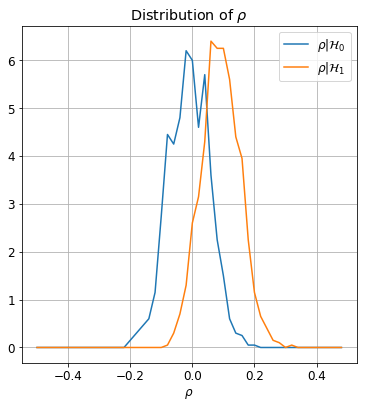
\includegraphics{output_2_0.png}
\caption{png}
\end{figure}

\begin{verbatim}
mean(rho|H0): 0.002
mean(rho|H1): 0.098
variance(rho|H0): 0.004
variance(rho|H1): 0.004
\end{verbatim}

As expected the variance of the two distribution is very similar
(asintoticaly is the same) as it depends only by the image size. Instead
the mean of \(\rho|\mathcal{H}_0\) depends from the intensity \(\gamma\)
of the watermark.

Using this information is now possible to compute the threshold \(\tau\)
as well as displaying the different probabilities depending on the
treshold.

\begin{verbatim}
tau: 0.050
Pf: 0.210
Pm: 0.209
Pd: 0.791
Pe: 0.420
\end{verbatim}

\begin{figure}
\centering
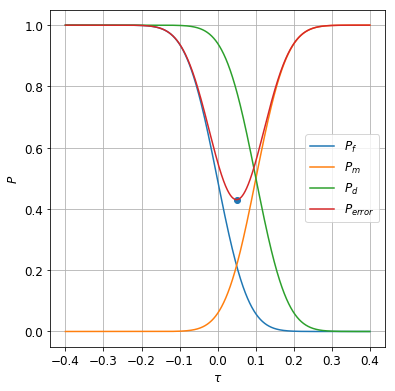
\includegraphics{output_5_1.png}
\caption{png}
\end{figure}

Using the Bayess hypotesis, the treshold \(\tau\) can be found in the
middle point (0.05) of the two distirbution (as the two hyptesis are
equiprobable and have same variance). This is also shown in the figure
above, as is in the middle point where the \(P_{error}\) is minimal.

The resulting probabilities are:

\begin{itemize}
\tightlist
\item
  \(P_f : 0.218\)
\item
  \(P_m : 0.219\)
\item
  \(P_d : 0.781\)
\end{itemize}

\paragraph{Exercise 1.2}\label{exercise-1.2}

In this exercise we were asked to evaluate the performance of the
\emph{Non-Blind} detector at different noise and watermark
configurations.

\begin{verbatim}
Variance(Noise): 50
-------------------
 - Theta: 0.1
   - Gamma: 1
        mean(rho|H0): -0.003
        mean(rho|H1): 0.096
        variance(rho|H0): 0.003
        variance(rho|H1): 0.003
   - Gamma: 5
        mean(rho|H0): 0.026
        mean(rho|H1): 2.512
        variance(rho|H0): 0.084
        variance(rho|H1): 0.091
 - Theta: 0.3
   - Gamma: 1
        mean(rho|H0): 0.001
        mean(rho|H1): 0.297
        variance(rho|H0): 0.011
        variance(rho|H1): 0.010
   - Gamma: 5
        mean(rho|H0): 0.027
        mean(rho|H1): 7.490
        variance(rho|H0): 0.280
        variance(rho|H1): 0.290

Variance(Noise): 100
-------------------
 - Theta: 0.1
   - Gamma: 1
        mean(rho|H0): 0.001
        mean(rho|H1): 0.091
        variance(rho|H0): 0.013
        variance(rho|H1): 0.014
   - Gamma: 5
        mean(rho|H0): -0.004
        mean(rho|H1): 2.477
        variance(rho|H0): 0.367
        variance(rho|H1): 0.410
 - Theta: 0.3
   - Gamma: 1
        mean(rho|H0): -0.021
        mean(rho|H1): 0.306
        variance(rho|H0): 0.048
        variance(rho|H1): 0.050
   - Gamma: 5
        mean(rho|H0): -0.009
        mean(rho|H1): 7.444
        variance(rho|H0): 1.025
        variance(rho|H1): 1.227
\end{verbatim}

The next table will summirize the results:

\begin{longtable}[]{@{}rrrrrrr@{}}
\toprule
\(\sigma^2_{noise}\) & \(\theta_N\) & \(\gamma\) & \$\mu\_\{\rho &
H\_0\}\$ & \$\sigma\^{}2\_\{\rho & H\_0\}\$\tabularnewline
\midrule
\endhead
50 & 0.1 & \(\pm1\) & 0.006 & 0.004 & 0.097 & 0.004\tabularnewline
50 & 0.1 & \(\pm5\) & 0.012 & 0.096 & 2.495 & 0.096\tabularnewline
50 & 0.3 & \(\pm1\) & 0.004 & 0.012 & 0.305 & 0.012\tabularnewline
50 & 0.3 & \(\pm5\) & -0.009 & 0.305 & 7.510 & 0.305\tabularnewline
100 & 0.1 & \(\pm1\) & 0.002 & 0.017 & 0.102 & 0.017\tabularnewline
100 & 0.1 & \(\pm5\) & 0.000 & 0.360 & 2.466 & 0.385\tabularnewline
100 & 0.3 & \(\pm1\) & 0.005 & 0.045 & 0.303 & 0.041\tabularnewline
100 & 0.3 & \(\pm5\) & 0.012 & 1.123 & 7.547 & 1.097\tabularnewline
\bottomrule
\end{longtable}

\begin{figure}
\centering
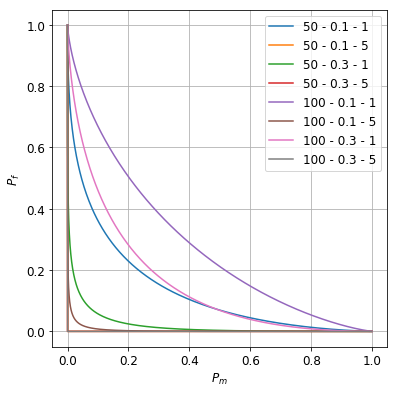
\includegraphics{output_10_0.png}
\caption{png}
\end{figure}

\begin{figure}
\centering
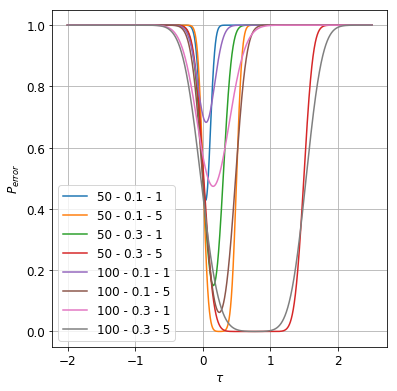
\includegraphics{output_10_1.png}
\caption{png}
\end{figure}

In conclusion the parameters control respectivly:

\begin{itemize}
\tightlist
\item
  \(\theta_N\): variate proportionally \(\mu_{\rho|H_1}\) and
  \(\sigma_\rho^2\)
\item
  \(\gamma\): variate quadratically \(\mu_{\rho|H_0}\) and
  \(\sigma_\rho^2\)
\item
  \(\sigma^2_{noise}\): variate quadratically \(\sigma_\rho^2\)
\end{itemize}

This is visualized in the following plots:

\begin{figure}
\centering
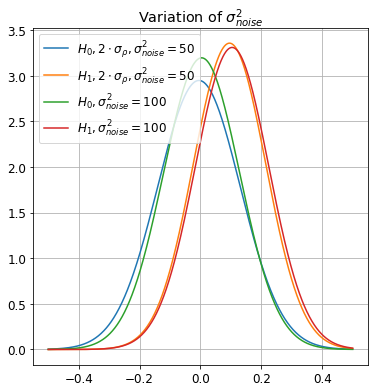
\includegraphics{output_12_0.png}
\caption{png}
\end{figure}

\begin{figure}
\centering
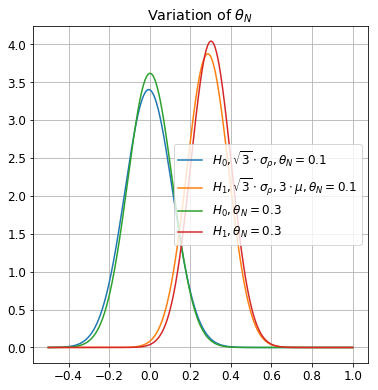
\includegraphics{output_12_1.png}
\caption{png}
\end{figure}

\begin{figure}
\centering
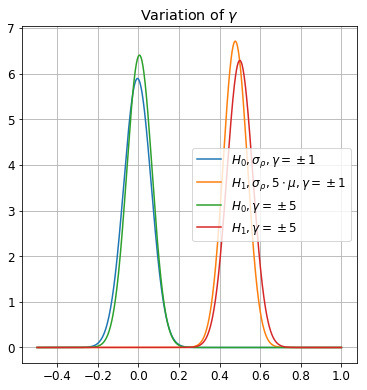
\includegraphics{output_12_2.png}
\caption{png}
\end{figure}

\subsection{Blind watermark detection}\label{blind-watermark-detection}

\paragraph{Exercise 2.1}\label{exercise-2.1}

In this exercise we will evaluate the performances of a blind watermark
detector using the same configuration than in the previous exercise.

The main difference (a very important one) is the fact that the detector
doesn't have access to the original image but instead have only the
watermarked noised one. To be able to extract the watermark, the host
image is extimated using a low pass filter (a median filter in my case).

\begin{verbatim}
Variance(Noise): 50
-------------------
 - Theta: 0.1
   - Gamma: 1
        mean(rho|H0): 0.003
        mean(rho|H1): 0.087
        variance(rho|H0): 0.004
        variance(rho|H1): 0.004
   - Gamma: 5
        mean(rho|H0): 0.002
        mean(rho|H1): 2.195
        variance(rho|H0): 0.088
        variance(rho|H1): 0.089
 - Theta: 0.3
   - Gamma: 1
        mean(rho|H0): 0.005
        mean(rho|H1): 0.262
        variance(rho|H0): 0.010
        variance(rho|H1): 0.012
   - Gamma: 5
        mean(rho|H0): 0.011
        mean(rho|H1): 6.613
        variance(rho|H0): 0.296
        variance(rho|H1): 0.276

Variance(Noise): 100
-------------------
 - Theta: 0.1
   - Gamma: 1
        mean(rho|H0): 0.014
        mean(rho|H1): 0.078
        variance(rho|H0): 0.014
        variance(rho|H1): 0.014
   - Gamma: 5
        mean(rho|H0): 0.033
        mean(rho|H1): 2.165
        variance(rho|H0): 0.335
        variance(rho|H1): 0.408
 - Theta: 0.3
   - Gamma: 1
        mean(rho|H0): -0.028
        mean(rho|H1): 0.260
        variance(rho|H0): 0.045
        variance(rho|H1): 0.043
   - Gamma: 5
        mean(rho|H0): 0.035
        mean(rho|H1): 6.635
        variance(rho|H0): 1.236
        variance(rho|H1): 1.002
\end{verbatim}

The next table will summirize the results:

\begin{longtable}[]{@{}rrrrrrr@{}}
\toprule
\(\sigma^2_{noise}\) & \(\theta_N\) & \(\gamma\) & \$\mu\_\{\rho &
H\_0\}\$ & \$\sigma\^{}2\_\{\rho & H\_0\}\$\tabularnewline
\midrule
\endhead
50 & 0.1 & \(\pm1\) & -0.017 & 0.003 & 0.082 & 0.004\tabularnewline
50 & 0.1 & \(\pm5\) & -0.025 & 0.098 & 2.215 & 0.094\tabularnewline
50 & 0.3 & \(\pm1\) & -0.013 & 0.010 & 0.261 & 0.010\tabularnewline
50 & 0.3 & \(\pm5\) & 0.134 & 0.305 & 6.583 & 0.305\tabularnewline
100 & 0.1 & \(\pm1\) & 0.009 & 0.014 & 0.085 & 0.014\tabularnewline
100 & 0.1 & \(\pm5\) & 0.082 & 0.327 & 2.280 & 0.316\tabularnewline
100 & 0.3 & \(\pm1\) & -0.011 & 0.043 & 0.266 & 0.041\tabularnewline
100 & 0.3 & \(\pm5\) & -0.007 & 1.064 & 6.561 & 1.164\tabularnewline
\bottomrule
\end{longtable}

\paragraph{Exercise 2.2}\label{exercise-2.2}

In this last exercise we will plot first the \emph{ROC} of the
\emph{Blind} detector and evaluate the performance differences with the
\emph{Non-Blind} one.

\begin{figure}
\centering
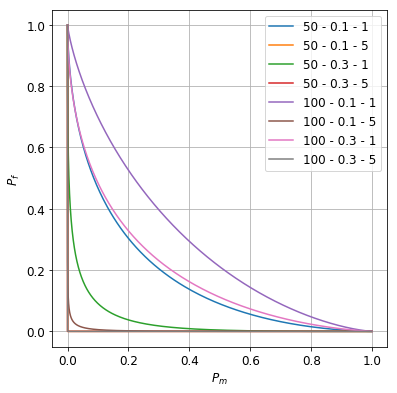
\includegraphics{output_17_0.png}
\caption{png}
\end{figure}

\begin{figure}
\centering
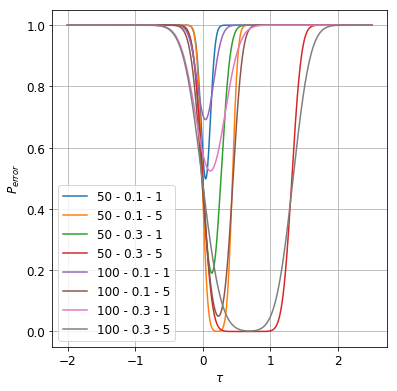
\includegraphics{output_17_1.png}
\caption{png}
\end{figure}

As it's possible to see the \emph{ROC} and the \(P_{error}\) plots are
both very similar to the \emph{Non-Blind} ones. The
\(\gamma\),\(\theta_N\) and \(\sigma^2_{noise}\) has the same impact of
before, however the fact that the original image is unkown has a small
impact on the \(\mu_{\rho|H_1}\), in average it is 12.9\% smaller, and
so close to \(\mu_{\rho|H_0}\), increasing the overall probability of
error.

The \(\sigma_\rho\) seems to decrease as well but less
(\textasciitilde{}6\%), and also the measure is more uncertain (the
variance is \textasciitilde{}10 times higher than the variance of the
avarage \(\mu_{\rho|H_1}\)).

Overall this small loss in performance doesn't impact to much in the
detection of the watermark and with smarter filtering it could be
possible to decrease the difference in performance between the two
systems.

\begin{verbatim}
Difference of mean between detectors: -12.9%
Variance: 0.069
Difference of sigma between detectors: -6.0%
Variance: 0.827
\end{verbatim}
